\subsection{Übung}

\subsubsection*{Aufgabe 8.1 (Modelle allgemein)}
    \paragraph*{Aufgabe}
        Nennen und beschreiben Sie die drei in der Vorlesung besprochenen Eigenschaften von Modellen.
    \paragraph*{Lösung}
        Partitionierung (Zerlegung des komplexen Sachverhaltes), Projektion (Betrachtung aus verschiedenen Perspektiven), Abstraktion (vernachlässigen unwichtiger Aspekte)

\subsubsection*{Aufgabe 8.2 (IST- und SOLL-Modelle)}
    \paragraph*{Aufgabe}
        \begin{enumerate}[label=\alph*)]
            \item Beschreiben Sie die Eigenschaften von IST- und SOLL-Modellen, indem Sie darauf eingehen, welchen Zustand eines zu modellierenden Sachverhalts die Modelle jeweils darstellen und welchem Charakter die Modelle dabei haben.
            \item Geben Sie ein Beispiel an, bei dem der Grundriss eines Hauses den Charakter eines SOLL-Modells hat.
            \item Geben Sie ein Beispiel an, bei dem der Grundriss eines Hauses den Charakter eines IST-Modells hat.
        \end{enumerate}
    \paragraph*{Lösung}
        \begin{enumerate}[label=\alph*)]
            \item IST-Modell: Zeigt den aktuellen Zustand (dokumentierend)SOLL-Modell: Zeigt den geplanten Zustand (entwerfend)
            \item Haus ist in der Planung (noch nicht gebaut)
            \item Haus ist gebaut
        \end{enumerate}

\subsubsection*{Aufgabe 8.3 (ARIS)}
    \paragraph*{Aufgabe}
        \begin{enumerate}[label=\alph*)]
            \item Nennen und beschreiben Sie die fünf Sichten von ARIS.
            \item Welche Gestaltungsebenen werden in der ARIS-Methode unterschieden? Beschreiben Sie den Fokus der genannten Gestaltungsebenen und deren Zusammenhänge.
            \item Inwiefern kommt der Steuerungssicht von ARIS eine besondere Rolle zu?
        \end{enumerate}
    \paragraph*{Lösung}
        \begin{enumerate}[label=\alph*)]
            \item 5 Sichten:
                \begin{itemize}
                    \item Organisationssicht: Darstellung der Aufbauorganisation, IT-Infrastruktur und Anwendungssysteme eines Betriebs.
                    \item Datensicht: Darstellung der verarbeiteten Daten im Unternehmen und deren Bedeutung für die Funktionen.
                    \item Steuerungssicht: Modellierung der ablaufenden Prozesse, Aktivitäten und Ereignisse im Unternehmen, verknüpft mit Organisations-, Daten- und Funktionssicht.
                    \item Funktionssicht: Darstellung der im Unternehmen auszuführenden Funktionen zur Erreichung operationalisierter Ziele.
                    \item Leistungssicht: Modellierung der vom Unternehmen zu erbringenden Leistungen, wie beispielsweise Produkte.
                \end{itemize}
            \item Gestaltungsebenen:
                \begin{itemize}
                    \item Fachkonzept: Fachliche Sicht, ohne technische Details.
                    \item DV-Konzept: Setzt das Fachkonzept technisch um, berücksichtigt IT-Details.
                    \item Implementierung: Realisiert das DV-Konzept durch Softwareentwicklung.
                \end{itemize}
            \item Ist die Zentrale Sicht, zeitliche Abfolge von Aktivitäten
        \end{enumerate}

\subsubsection*{Aufgabe 8.4 (ER-Modell: Bestellanforderung)}
    \paragraph*{Aufgabe}
        Erstellen Sie ein ER-Modell zur Konkretisierung von Bestellanforderungen, das den nachfolgend beschriebenen Anforderungen entspricht:
        Zu einer Bestellanforderung sind das Erstellungsdatum und der Bedarfsträger (Name und Personalnummer) zu erfassen. Außerdem sind die Materialien zu erfassen, auf die sich die Bestellanforderung bezieht. Ein Material wird dabei durch die Materialnummer eindeutig beschrieben. Zusätzlich sind der Name, das Abmaß und das Gewicht des Materials zu erfassen und es ist anzugeben, in welcher Menge ein Material zu bestellen ist. Sehen Sie für die Bestellanforderung und für den Bedarfsträger geeignete Primärschlüssel vor und vergessen Sie nicht, die Beziehung durch die Angabe von Kardinalitäten geeignet einzuschränken.

        \begin{figure}[h]
            \centering
            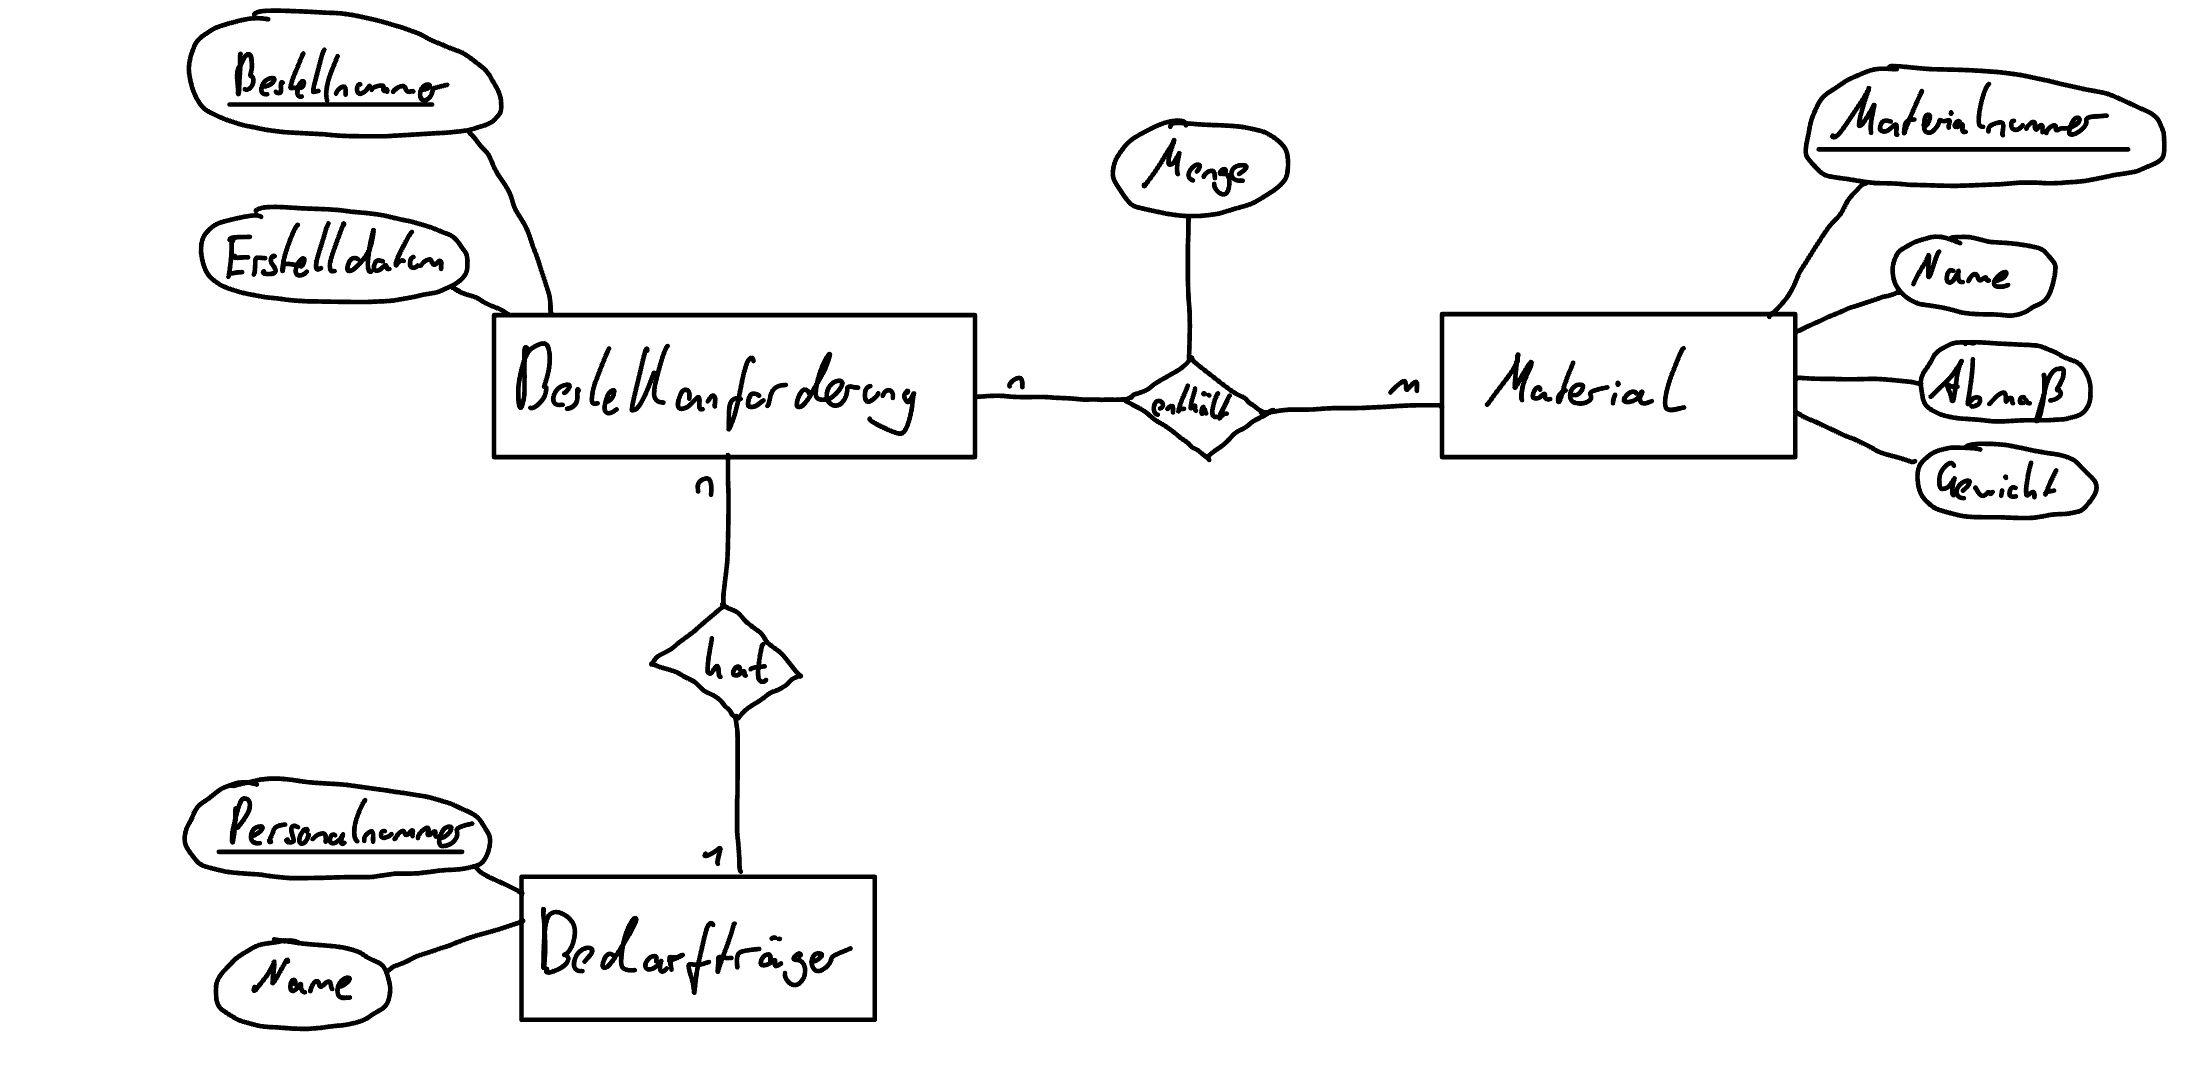
\includegraphics[width=\textwidth]{image/ER-Modell.png}
            \caption{Lösung Aufgabe 8.4 (ER-Modell: Bestellanforderung)}
            \label{fig:ER-Modell}
        \end{figure}